\section{Thiết lập thực nghiệm}

\subsection{Khu vực nghiên cứu}

\textbf{Lưu ý về địa giới hành chính:} Theo Nghị quyết số 1278/NQ-UBTVQH15 ngày 24/10/2024 của Ủy ban Thường vụ Quốc hội, kể từ ngày 01/07/2025, tỉnh Cà Mau và tỉnh Bạc Liêu được sáp nhập thành tỉnh Cà Mau mới với tổng diện tích tự nhiên 7,942.38 km² và dân số khoảng 2.6 triệu người. Đồ án này nghiên cứu trên phạm vi rừng của tỉnh Cà Mau mới, bao gồm cả vùng rừng thuộc địa bàn Bạc Liêu cũ.

Tỉnh Cà Mau mới nằm ở cực Nam Tổ Quốc, sở hữu hệ sinh thái rừng đa dạng bao gồm cả rừng ngập mặn ven biển và rừng tràm nội địa. Theo số liệu trước khi sáp nhập, tỉnh Cà Mau cũ có diện tích rừng khoảng 94,319 hecta và tỉnh Bạc Liêu có khoảng 5,730 hecta rừng, tổng cộng khoảng 100,000 hecta rừng trên toàn tỉnh Cà Mau mới \citevi{snnptntcamau2021}. Trong đó, rừng ngập mặn Cà Mau chiếm khoảng 20\% diện tích rừng ngập mặn của Việt Nam. Hệ thống rừng tại Cà Mau đóng vai trò then chốt trong việc phòng hộ ven biển (chắn sóng, chống xâm thực và bảo vệ bờ biển), bảo tồn đa dạng sinh học vì là môi trường sống cho nhiều loài động thực vật quý hiếm, cung cấp nguồn sinh kế thông qua các hoạt động thủy sản và du lịch sinh thái, và góp phần giảm nhẹ biến đổi khí hậu nhờ khả năng lưu giữ carbon cao, gấp khoảng 3–5 lần so với rừng nhiệt đới trên cạn \citeen{donato2011,alongi2014}.

Tuy nhiên, rừng Cà Mau đang phải đối mặt với nhiều thách thức. Trước hết là áp lực chuyển đổi sang nuôi tôm do kinh tế, khiến nhiều khu vực rừng bị chuyển đổi thành ao nuôi. Ngoài ra, hiện tượng xâm nhập mặn gia tăng do biến đổi khí hậu làm giảm sức khỏe rừng; đồng thời xói mòn bờ biển cũng làm suy giảm diện tích rừng ven biển; và tình trạng thiếu nước ngọt ảnh hưởng tới khả năng tái sinh tự nhiên của rừng. Giai đoạn 2011-2023, sạt lở vùng ven biển đã làm mất hơn 6,200 hecta đất và rừng phòng hộ \citevi{nongnghiepmoitruong2024}.

\begin{figure}[H]
    \centering
    \includegraphics[width=0.95\textwidth]{img/chapter1/LULC-Ca-Mau.png}
    \caption{Bản đồ lớp phủ bề mặt khu vực tỉnh Cà Mau.}
    \label{fig:camau_lulc}
\end{figure}

Đồ án tập trung vào toàn bộ vùng quy hoạch lâm nghiệp của tỉnh Cà Mau mới. Dữ liệu ranh giới quy hoạch lâm nghiệp được cung cấp bởi Công ty TNHH Tư vấn và Phát triển Đồng Xanh — đối tác của Chi cục Kiểm lâm tỉnh Cà Mau.

\begin{figure}[H]
    \centering
    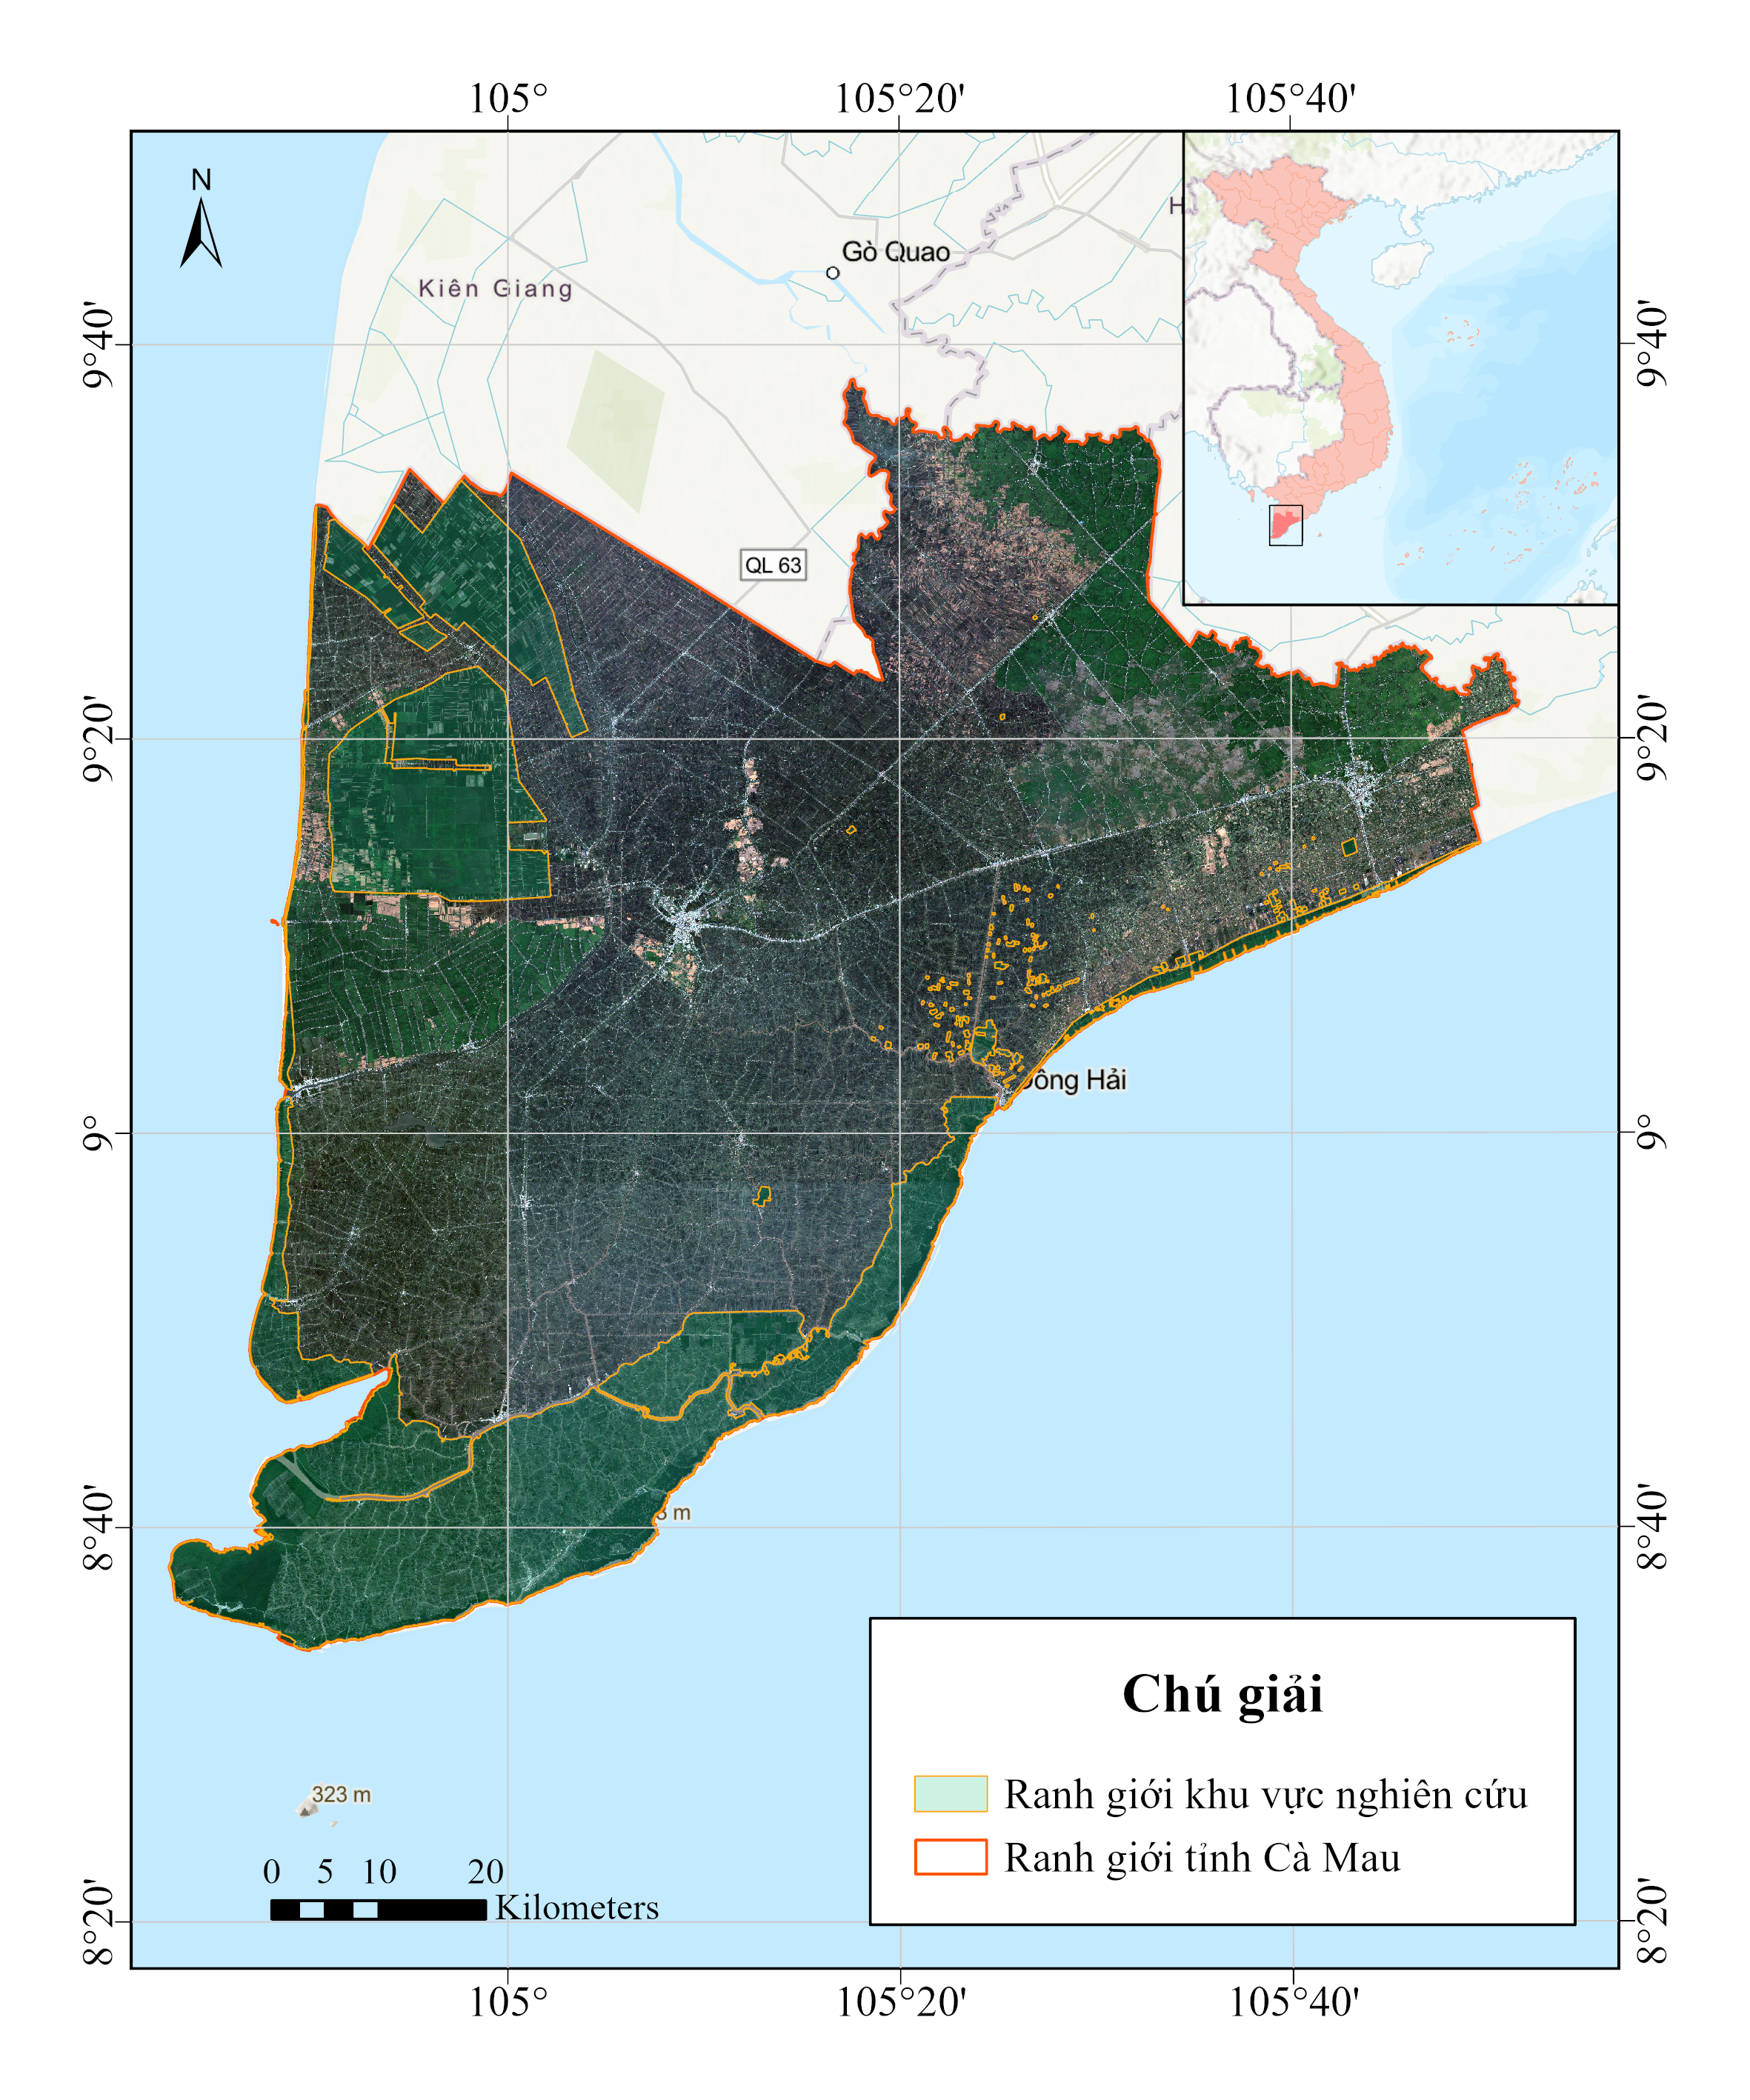
\includegraphics[width=0.95\textwidth]{img/chapter1/RGB-Ca-Mau.png}
    \caption{Ảnh vệ tinh tổ hợp màu tự nhiên (RGB) khu vực nghiên cứu tỉnh Cà Mau.}
    \label{fig:study_area}
\end{figure}

Tổng diện tích ranh giới quy hoạch là 170,178.82 hecta (tương đương 1,701.79 km²), bao gồm 666 polygon trong file shapefile ranh giới. Diện tích thực tế được phân loại là 162,468.50 hecta (khoảng 95.5\% diện tích ranh giới); phần còn lại (~7,710 ha, chiếm 4.5\%) bị loại do mây che phủ hoặc dữ liệu không hợp lệ (nodata) trong quá trình xử lý ảnh vệ tinh. Kích thước raster là 12,547 × 10,917 pixels (ở độ phân giải 10m), sử dụng hệ quy chiếu EPSG:32648 (WGS 84 / UTM Zone 48N).

\subsection{Dữ liệu thực địa tại Cà Mau}

Dữ liệu thực địa được thu thập thông qua quy trình khảo sát chuyên nghiệp với sự phối hợp giữa Chi cục Kiểm lâm tỉnh Cà Mau và Công ty TNHH Tư vấn và Phát triển Đồng Xanh (GFD). Quy trình thu thập gồm ba giai đoạn. Giai đoạn đầu tiên là khảo sát thực địa bằng thiết bị bay không người lái (drone) để ghi nhận hình ảnh và xác định trạng thái rừng. Giai đoạn thứ hai là số hóa các điểm dữ liệu thực địa trên phần mềm QGIS, đối chiếu với ảnh vệ tinh Sentinel-2. Giai đoạn cuối cùng là kiểm tra chéo và loại bỏ các điểm không rõ ràng hoặc nằm trong vùng mây che phủ.

Dữ liệu cuối cùng được xuất dưới dạng file CSV với cấu trúc gồm 4 trường: \texttt{id}, \texttt{label}, \texttt{x} và \texttt{y} (tọa độ theo hệ quy chiếu EPSG:32648).

\begin{table}[H]
\centering
\caption{Thống kê dữ liệu thực địa theo lớp biến động}
\label{tab:ground_truth}
\begin{tabular}{|c|l|c|c|l|}
\hline
\textbf{Lớp} & \textbf{Tên} & \textbf{Số điểm} & \textbf{Tỷ lệ} & \textbf{Mô tả} \\
\hline
0 & Rừng ổn định & 656 & 24.9\% & Có rừng ở cả 2 kỳ \\
\hline
1 & Mất rừng & 650 & 24.7\% & Có rừng $\rightarrow$ không có rừng \\
\hline
2 & Phi rừng & 664 & 25.3\% & Không có rừng ở cả 2 kỳ \\
\hline
3 & Phục hồi rừng & 660 & 25.1\% & Không có $\rightarrow$ có rừng \\
\hline
\textbf{Tổng} & & \textbf{2,630} & \textbf{100\%} & Phân bố cân bằng \\
\hline
\end{tabular}
\end{table}

Phân bố không gian của các điểm dữ liệu thực địa được minh họa trong Hình~\ref{fig:ground_truth_map}. Các điểm mẫu được thu thập phân tán trên toàn bộ khu vực nghiên cứu, đảm bảo tính đại diện về mặt không gian cho các loại hình biến động rừng khác nhau.

\begin{figure}[H]
\centering
\includegraphics[width=0.9\textwidth]{chapter3/samples.png}
\caption{Bản đồ phân bố không gian các điểm dữ liệu thực địa trên khu vực nghiên cứu tỉnh Cà Mau}
\label{fig:ground_truth_map}
\end{figure}

\subsection{Cấu hình phần cứng và phần mềm}

Môi trường thí nghiệm gồm phần cứng như GPU NVIDIA GeForce RTX 4080 (16GB VRAM), bộ nhớ RAM 64GB và bộ nhớ lưu trữ 1TB SSD. Về phần mềm, hệ thống sử dụng Python 3.8 trở lên cùng PyTorch 2.0+ có hỗ trợ CUDA để huấn luyện mô hình, GDAL 3.4+ cho xử lý dữ liệu không gian và các thư viện khoa học dữ liệu như NumPy, scikit-learn và pandas.

\subsection{Phân chia dữ liệu}

Bộ dữ liệu thực địa gồm 2,630 điểm, trong đó phân bố lớp gần như cân bằng: Lớp 0 (Rừng ổn định) 656 điểm (24.94\%), Lớp 1 (Mất rừng) 650 điểm (24.71\%), Lớp 2 (Phi rừng) 664 điểm (25.25\%) và Lớp 3 (Phục hồi rừng) 660 điểm (25.10\%).

\begin{table}[H]
\centering
\caption{Phân bố dữ liệu theo tập huấn luyện và kiểm tra}
\label{tab:data_split_info}
\begin{tabular}{|l|c|c|}
\hline
\textbf{Tập dữ liệu} & \textbf{Số mẫu} & \textbf{Tỷ lệ} \\
\hline
Training + Validation (5-Fold CV) & 2,104 & 80\% \\
\hline
Test (cố định) & 526 & 20\% \\
\hline
\textbf{Tổng} & \textbf{2,630} & \textbf{100\%} \\
\hline
\end{tabular}
\end{table}

Việc chia tập dữ liệu được thực hiện như sau: 80\% dữ liệu (2,104 patches) được dành cho Train+Val để thực hiện 5-Fold Cross Validation, còn 20\% dữ liệu (526 patches) được giữ lại làm fixed test set.
